% questions.tex —— 2018 年·江苏卷 · 题目内容片段（无答案）
% 由 tools/generate_projects.py 依来源总账自 2018/2018_数学真题_江苏_试题.md 生成，勿手改（改源 MD 后重跑）

\begin{gktip}
来源：固定来源 \texttt{src-b98d418cc401881ac96eba763226a8709b29e353718dc5dfb35fd7929bbf57af}（\texttt{普通高考/2018/2018江苏.pdf}，原卷印刷页 1065—1066）。
声明：内部绑定只固定输入字节，不认证出版者、版次、上游来源链及官方身份；固定源不附答案页。
\end{gktip}

\par\medskip

\gkpart{一、填空题}

\begin{question}
\gkti{1}已知集合 $A = \{0, 1, 2, 8\}$，$B = \{-1, 1, 6, 8\}$，那么 $A \cap B =$\gkblank{}。

\end{question}
\begin{question}
\gkti{2}若复数 $z$ 满足 $\mathrm{i} \cdot z = 1 + 2\mathrm{i}$，其中 $\mathrm{i}$ 是虚数单位，则 $z$ 的实部为\gkblank{}。

\Needspace{0.4\textheight}
\end{question}
\begin{question}
\gkti{3}已知 5 位裁判给某运动员打出的分数的茎叶图如图所示，那么这 5 位裁判打出的分数的平均数为\gkblank{}。
\nopagebreak[4]
\begin{center}% 2018 江苏卷第3题：裁判打分茎叶图
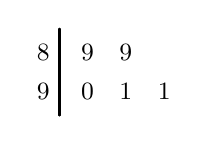
\begin{tikzpicture}[font=\small, line cap=round, line join=round]
  \node[left] at (0, 0.5) {$8$};
  \node[left] at (0, 0) {$9$};
  \draw[thick] (0, 0.8) -- (0, -0.3);
  \node[right] at (0.15, 0.5) {$9\quad 9$};
  \node[right] at (0.15, 0) {$0\quad 1\quad 1$};
\end{tikzpicture}
\end{center}
\nopagebreak[4]
\Needspace{0.4\textheight}
\end{question}
\begin{question}
\gkti{4}一个算法的伪代码如图所示，执行此算法，最后输出的 $S$ 的值为\gkblank{}。
\nopagebreak[4]
\begin{center}% 2018 江苏卷第4题：算法伪代码框
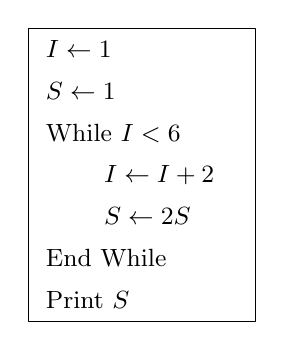
\begin{tikzpicture}[line cap=round,line join=round,font=\small,x=0.03515cm,y=0.03515cm]
\draw (0,0) rectangle (82,106);
\node[anchor=base west,inner sep=0] at (6.18,95.46) {\(I\leftarrow 1\)};
\node[anchor=base west,inner sep=0] at (6.18,80.34) {\(S\leftarrow 1\)};
\node[anchor=base west,inner sep=0] at (6.18,65.22) {While \(I<6\)};
\node[anchor=base west,inner sep=0] at (27.18,50.10) {\(I\leftarrow I+2\)};
\node[anchor=base west,inner sep=0] at (27.18,34.98) {\(S\leftarrow 2S\)};
\node[anchor=base west,inner sep=0] at (6.18,19.86) {End While};
\node[anchor=base west,inner sep=0] at (6.18,4.74) {Print \(S\)};
\end{tikzpicture}
\end{center}
\nopagebreak[4]
\end{question}
\begin{question}
\gkti{5}函数 $f(x) = \sqrt{\log_2 x - 1}$ 的定义域为\gkblank{}。

\end{question}
\begin{question}
\gkti{6}某兴趣小组有 2 名男生和 3 名女生，现从中任选 2 名学生去参加活动，则恰好选中 2 名女生的概率为\gkblank{}。

\end{question}
\begin{question}
\gkti{7}已知函数 $y = \sin(2x + \varphi)$ $\left(-\dfrac{\pi}{2} < \varphi < \dfrac{\pi}{2}\right)$ 的图象关于直线 $x = \dfrac{\pi}{3}$ 对称，则 $\varphi$ 的值为\gkblank{}。

\end{question}
\begin{question}
\gkti{8}在平面直角坐标系 $xOy$ 中，若双曲线 $\dfrac{x^2}{a^2} - \dfrac{y^2}{b^2} = 1$ ($a > 0, b > 0$) 的右焦点 $F(c, 0)$ 到一条渐近线的距离为 $\dfrac{\sqrt{3}}{2}c$，则其离心率的值为\gkblank{}。

\end{question}
\begin{question}
\gkti{9}函数 $f(x)$ 满足 $f(x + 4) = f(x)$ ($x \in \mathbf{R}$)，且在区间 $(-2, 2]$ 上，
\nopagebreak[4]
\[f(x) = \begin{cases} \cos\dfrac{\pi x}{2}, & 0 < x \leqslant 2, \\ x + \dfrac{1}{2}, & -2 < x \leqslant 0, \end{cases}\]
则 $f(f(15))$ 的值为\gkblank{}。

\Needspace{0.4\textheight}
\end{question}
\begin{question}
\gkti{10}如图所示，正方体的棱长为 2，以其所有面的中心为顶点的多面体的体积为\gkblank{}。
\nopagebreak[4]
\begin{center}% 2018 江苏卷第10题：正方体中心多面体（正八面体）
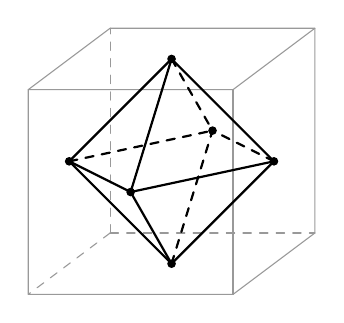
\begin{tikzpicture}[font=\small, line cap=round, line join=round, >=stealth, scale=1.3]
  % 正方体顶点
  \coordinate (A) at (0, 0);
  \coordinate (B) at (2, 0);
  \coordinate (C) at (2.8, 0.6);
  \coordinate (D) at (0.8, 0.6);
  \coordinate (A1) at (0, 2);
  \coordinate (B1) at (2, 2);
  \coordinate (C1) at (2.8, 2.6);
  \coordinate (D1) at (0.8, 2.6);

  % 六个面中心
  \coordinate (F_front) at (1, 1);
  \coordinate (F_back) at (1.8, 1.6);
  \coordinate (F_left) at (0.4, 1.3);
  \coordinate (F_right) at (2.4, 1.3);
  \coordinate (F_bottom) at (1.4, 0.3);
  \coordinate (F_top) at (1.4, 2.3);

  % 正方体虚线棱
  \draw[dashed, thin, gray!80] (D) -- (A);
  \draw[dashed, thin, gray!80] (D) -- (C);
  \draw[dashed, thin, gray!80] (D) -- (D1);

  % 正方体实线棱
  \draw[thin, gray!80] (A) -- (B) -- (C) -- (C1) -- (D1) -- (A1) -- cycle;
  \draw[thin, gray!80] (B) -- (B1);
  \draw[thin, gray!80] (A1) -- (B1) -- (C1);

  % 多面体虚线棱（连接后部和内部的中心）
  \draw[dashed, thick] (F_top) -- (F_back);
  \draw[dashed, thick] (F_bottom) -- (F_back);
  \draw[dashed, thick] (F_left) -- (F_back);
  \draw[dashed, thick] (F_right) -- (F_back);

  % 多面体实线棱
  \draw[thick] (F_top) -- (F_front);
  \draw[thick] (F_top) -- (F_left);
  \draw[thick] (F_top) -- (F_right);
  \draw[thick] (F_bottom) -- (F_front);
  \draw[thick] (F_bottom) -- (F_left);
  \draw[thick] (F_bottom) -- (F_right);
  \draw[thick] (F_front) -- (F_left);
  \draw[thick] (F_front) -- (F_right);

  % 各中心点标记
  \foreach \p in {F_front, F_back, F_left, F_right, F_bottom, F_top} {
    \fill (\p) circle (1.2pt);
  }
\end{tikzpicture}
\end{center}
\nopagebreak[4]
\end{question}
\begin{question}
\gkti{11}若函数 $f(x) = 2x^3 - ax^2 + 1$ ($a \in \mathbf{R}$) 在 $(0, +\infty)$ 内有且只有一个零点，则 $f(x)$ 在 $[-1, 1]$ 上的最大值与最小值的和为\gkblank{}。

\end{question}
\begin{question}
\gkti{12}在平面直角坐标系 $xOy$ 中，$A$ 为直线 $l: y = 2x$ 上在第一象限内的点，$B(5, 0)$，以 $AB$ 为直径的圆 $C$ 与直线 $l$ 交于另一点 $D$。若 $\overrightarrow{AB} \cdot \overrightarrow{CD} = 0$，则点 $A$ 的横坐标为\gkblank{}。

\end{question}
\begin{question}
\gkti{13}在 $\triangle ABC$ 中，角 $A, B, C$ 所对的边分别为 $a, b, c$，$\angle ABC = 120^\circ$，$\angle ABC$ 的平分线交 $AC$ 于点 $D$，且 $BD = 1$，则 $4a + c$ 的最小值为\gkblank{}。

\end{question}
\begin{question}
\gkti{14}已知集合 $A = \{x \mid x = 2n - 1, n \in \mathbf{N}^*\}$，$B = \{x \mid x = 2^n, n \in \mathbf{N}^*\}$。将 $A \cup B$ 的所有元素从小到大依次排列构成一个数列 $\{a_n\}$。记 $S_n$ 为数列 $\{a_n\}$ 的前 $n$ 项和，则使得 $S_n > 12a_{n+1}$ 成立的 $n$ 的最小值为\gkblank{}。

\end{question}
\gkpart{二、解答题}

\Needspace{0.4\textheight}
\begin{question}
\gkti{15}在平行六面体 $ABCD - A_1B_1C_1D_1$ 中，$AA_1 = AB$，$AB_1 \perp B_1C_1$。求证：

（1） $AB \parallel$ 平面 $A_1B_1C$；

（2） 平面 $ABB_1A_1 \perp$ 平面 $A_1BC$。
\nopagebreak[4]
\begin{center}% 2018 江苏卷第15题：平行六面体 ABCD-A1B1C1D1
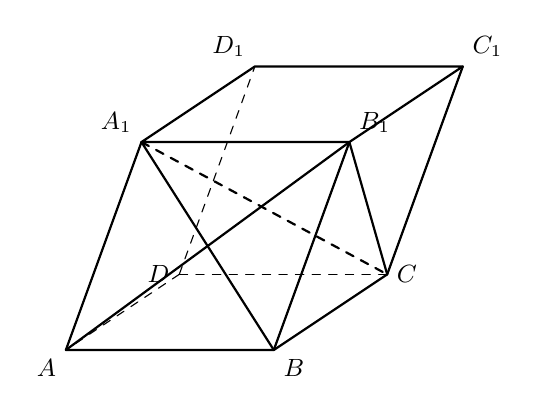
\begin{tikzpicture}[font=\small, line cap=round, line join=round, >=stealth, scale=1.2]
  % 顶点坐标
  \coordinate (A) at (0, 0);
  \coordinate (B) at (2.2, 0);
  \coordinate (C) at (3.4, 0.8);
  \coordinate (D) at (1.2, 0.8);
  \coordinate (A1) at (0.8, 2.2);
  \coordinate (B1) at (3.0, 2.2);
  \coordinate (C1) at (4.2, 3.0);
  \coordinate (D1) at (2.0, 3.0);

  % 隐藏棱（虚线）
  \draw[dashed, thin] (D) -- (A);
  \draw[dashed, thin] (D) -- (C);
  \draw[dashed, thin] (D) -- (D1);
  \draw[dashed, thick] (A1) -- (C);

  % 可见棱（实线）
  \draw[thick] (A) -- (B) -- (C);
  \draw[thick] (A1) -- (B1) -- (C1) -- (D1) -- cycle;
  \draw[thick] (A) -- (A1);
  \draw[thick] (B) -- (B1);
  \draw[thick] (C) -- (C1);

  % 辅助线/对角线
  \draw[thick] (A) -- (B1);
  \draw[thick] (A1) -- (B);
  \draw[thick] (B1) -- (C);

  % 顶点标签
  \node[below left] at (A) {$A$};
  \node[below right] at (B) {$B$};
  \node[right] at (C) {$C$};
  \node[left] at (D) {$D$};
  \node[above left] at (A1) {$A_1$};
  \node[above right] at (B1) {$B_1$};
  \node[above right] at (C1) {$C_1$};
  \node[above left] at (D1) {$D_1$};
\end{tikzpicture}
\end{center}
\nopagebreak[4]
\end{question}
\begin{question}
\gkti{16}已知 $\alpha, \beta$ 为锐角，$\tan\alpha = \dfrac{4}{3}$，$\cos(\alpha + \beta) = -\dfrac{\sqrt{5}}{5}$。

（1） 求 $\cos 2\alpha$ 的值；

（2） 求 $\tan(\alpha - \beta)$ 的值。

\Needspace{0.4\textheight}
\end{question}
\begin{question}
\gkti{17}某农场有一块农田，如图所示，它的边界由圆 $O$ 的一段圆弧 $MPN$（$P$ 为此圆弧的中点）和线段 $MN$ 构成。已知圆 $O$ 的半径为 40 米，点 $P$ 到 $MN$ 的距离为 50 米。现规划在此农田上修建两个温室大棚，大棚 I 内的地块形状为矩形 $ABCD$，大棚 II 内的地块形状为 $\triangle CDP$，要求 $A, B$ 均在线段 $MN$ 上，$C, D$ 均在圆弧上。设 $OC$ 与 $MN$ 所成的角为 $\theta$。

（1） 用 $\theta$ 分别表示矩形 $ABCD$ 和 $\triangle CDP$ 的面积，并确定 $\sin\theta$ 的取值范围；

（2） 若大棚 I 内种植甲种蔬菜，大棚 II 内种植乙种蔬菜，且甲、乙两种蔬菜的单位面积年产值之比为 $4 : 3$。求当 $\theta$ 为何值时，能使甲、乙两种蔬菜的年总产值最大。
\nopagebreak[4]
\begin{center}% 2018 江苏卷第17题：农田大棚温室几何图
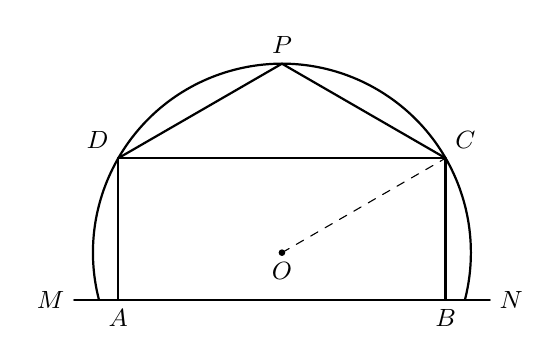
\begin{tikzpicture}[font=\small, line cap=round, line join=round, >=stealth, scale=0.06]
  % 圆心与原点
  \coordinate (O) at (0, 0);
  \coordinate (P) at (0, 40);
  \coordinate (M) at (-44, -10);
  \coordinate (N) at (44, -10);

  % 绘制底边线段 MN
  \draw[thick] (M) -- (N);

  % 绘制圆弧 MPN
  \draw[thick] (-38.73, -10) arc (194.48: -14.48: 40);

  % 矩形 ABCD
  \coordinate (C) at (34.64, 20);
  \coordinate (D) at (-34.64, 20);
  \coordinate (B) at (34.64, -10);
  \coordinate (A) at (-34.64, -10);

  \draw[thick] (A) -- (B) -- (C) -- (D) -- cycle;

  % 三角形 CDP
  \draw[thick] (D) -- (P) -- (C);

  % 连结 OC
  \draw[dashed] (O) -- (C);

  % 标记点与标签
  \fill (O) circle (20pt) node[below] {$O$};
  \node[above] at (P) {$P$};
  \node[above left] at (D) {$D$};
  \node[above right] at (C) {$C$};
  \node[left] at (M) {$M$};
  \node[right] at (N) {$N$};
  \node[below] at (A) {$A$};
  \node[below] at (B) {$B$};
\end{tikzpicture}
\end{center}
\nopagebreak[4]
\Needspace{0.4\textheight}
\end{question}
\begin{question}
\gkti{18}如图，在平面直角坐标系 $xOy$ 中，椭圆 $C$ 过点 $\left(\sqrt{3}, \dfrac{1}{2}\right)$，焦点为 $F_1(-\sqrt{3}, 0)$，$F_2(\sqrt{3}, 0)$，圆 $O$ 的直径为 $F_1F_2$。

（1） 求椭圆 $C$ 及圆 $O$ 的方程；

（2） 设直线 $l$ 与圆 $O$ 相切于第一象限内的点 $P$。
① 若直线 $l$ 与椭圆 $C$ 有且只有一个公共点，求点 $P$ 的坐标；
② 直线 $l$ 与椭圆 $C$ 交于 $A, B$ 两点。若 $\triangle OAB$ 的面积为 $\dfrac{2\sqrt{6}}{7}$，求直线 $l$ 的方程。
\nopagebreak[4]
\begin{center}% 2018 江苏卷第18题：椭圆与焦点直径圆
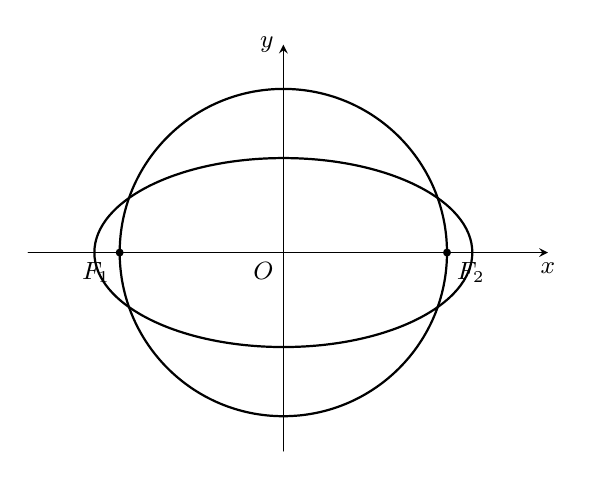
\begin{tikzpicture}[font=\small, line cap=round, line join=round, >=stealth, scale=1.2]
  % 坐标轴
  \draw[->] (-2.7, 0) -- (2.8, 0) node[below] {$x$};
  \draw[->] (0, -2.1) -- (0, 2.2) node[left] {$y$};
  \node[below left] at (0, 0) {$O$};

  % 椭圆: x^2/4 + y^2 = 1 (a=2, b=1)
  \draw[thick] (0, 0) ellipse (2cm and 1cm);

  % 圆: x^2 + y^2 = 3 (r = sqrt(3) ≈ 1.732)
  \draw[thick] (0, 0) circle (1.732cm);

  % 焦点 F1(-sqrt(3), 0), F2(sqrt(3), 0)
  \coordinate (F1) at (-1.732, 0);
  \coordinate (F2) at (1.732, 0);
  \fill (F1) circle (1.2pt) node[below left] {$F_1$};
  \fill (F2) circle (1.2pt) node[below right] {$F_2$};
\end{tikzpicture}
\end{center}
\nopagebreak[4]
\end{question}
\begin{question}
\gkti{19}记 $f'(x), g'(x)$ 分别为函数 $f(x), g(x)$ 的导函数。若存在 $x_0 \in \mathbf{R}$，满足 $f(x_0) = g(x_0)$ 且 $f'(x_0) = g'(x_0)$，则称 $x_0$ 为函数 $f(x)$ 与 $g(x)$ 的一个“S 点”。

（1） 证明：函数 $f(x) = x$ 与 $g(x) = x^2 + 2x - 2$ 不存在“S 点”；

（2） 若函数 $f(x) = ax^2 - 1$ 与 $g(x) = \ln x$ 存在“S 点”，求实数 $a$ 的值；

（3） 已知函数 $f(x) = -x^2 + a$，$g(x) = \dfrac{b\mathrm{e}^x}{x}$。对任意 $a > 0$，判断是否存在 $b > 0$，使函数 $f(x)$ 与 $g(x)$ 在区间 $(0, +\infty)$ 内存在“S 点”，并说明理由。

\end{question}
\begin{question}
\gkti{20}设 $\{a_n\}$ 是首项为 $a_1$，公差为 $d$ 的等差数列，$\{b_n\}$ 是首项为 $b_1$，公比为 $q$ 的等比数列。

（1） 设 $a_1 = 0$，$b_1 = 1$，$q = 2$，若 $|a_n - b_n| \leqslant b_1$ 对 $n = 1, 2, 3, 4$ 均成立，求 $d$ 的取值范围；

（2） 若 $a_1 = b_1 > 0$，$m \in \mathbf{N}^*$，$q \in \left(1, \sqrt[m]{2}\right]$，证明：存在 $d \in \mathbf{R}$，使得 $|a_n - b_n| \leqslant b_1$ 对 $n = 2, 3, \cdots, m + 1$ 均成立，并求 $d$ 的取值范围（用 $b_1, m, q$ 表示）。

\Needspace{0.4\textheight}
\end{question}
\begin{question}
\gkti{21}四选二。

【A】如图，圆 $O$ 的半径为 2，$AB$ 为圆 $O$ 的直径，$P$ 为 $AB$ 延长线上一点，过 $P$ 作圆 $O$ 的切线，切点为 $C$。若 $PC = 2\sqrt{3}$，求 $BC$ 的长。
\nopagebreak[4]
\begin{center}% 2018 江苏卷第21题【A】：圆切线与割线
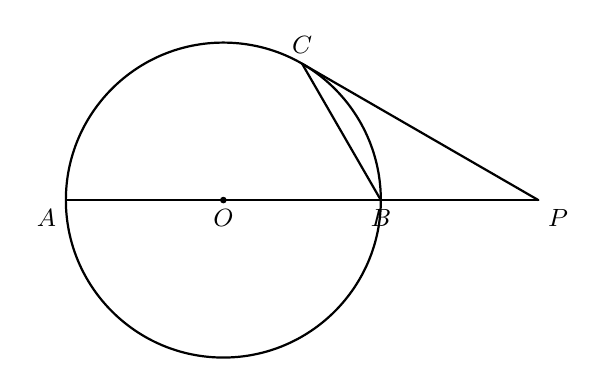
\begin{tikzpicture}[font=\small, line cap=round, line join=round, >=stealth, scale=1.0]
  % 圆心与半径 R = 2
  \coordinate (O) at (0, 0);
  \draw[thick] (O) circle (2cm);

  % 直径 AB: A(-2, 0), B(2, 0)
  \coordinate (A) at (-2, 0);
  \coordinate (B) at (2, 0);

  % P 在 AB 延长线上，P(4, 0)
  \coordinate (P) at (4, 0);
  \draw[thick] (A) -- (P);

  % 切点 C: (1, sqrt(3))
  \coordinate (C) at (1, 1.732);

  % 切线 PC 与 弦 BC
  \draw[thick] (P) -- (C);
  \draw[thick] (B) -- (C);

  % 标签与点
  \fill (O) circle (1.2pt) node[below] {$O$};
  \node[below left] at (A) {$A$};
  \node[below] at (B) {$B$};
  \node[below right] at (P) {$P$};
  \node[above] at (C) {$C$};
\end{tikzpicture}
\end{center}
\nopagebreak[4]
【B】已知矩阵 $A = \begin{bmatrix} 2 & 3 \\ 1 & 2 \end{bmatrix}$。（1）求 $A$ 的逆矩阵 $A^{-1}$；（2）若点 $P$ 在矩阵 $A$ 对应的变换作用下得到点 $P'(3, 1)$，求点 $P$ 的坐标。

【C】在极坐标系中，直线 $l$ 的方程为 $\rho \sin\left(\dfrac{\pi}{6} - \theta\right) = 2$，曲线 $C$ 的方程为 $\rho = 4\cos\theta$，求直线 $l$ 被曲线 $C$ 截得的弦长。

【D】若 $x, y, z$ 为实数，且 $x + 2y + 2z = 6$，求 $x^2 + y^2 + z^2$ 的最小值。

\Needspace{0.4\textheight}
\end{question}
\begin{question}
\gkti{22}如图，在正三棱柱 $ABC - A_1B_1C_1$ 中，$AB = AA_1 = 2$，点 $P, Q$ 分别为 $A_1B_1, BC$ 的中点。

（1） 求异面直线 $BP$ 与 $AC_1$ 所成角的余弦值；

（2） 求直线 $CC_1$ 与平面 $AQC_1$ 所成角的正弦值。
\nopagebreak[4]
\begin{center}% 2018 江苏卷第22题：正三棱柱 ABC-A1B1C1
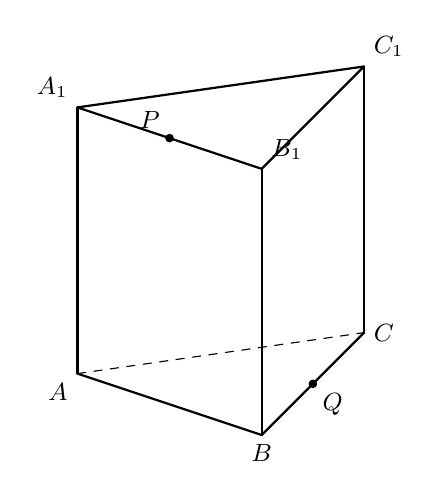
\begin{tikzpicture}[font=\small, line cap=round, line join=round, >=stealth, scale=1.3]
  % 底面顶点 A, B, C
  \coordinate (A) at (0, 0);
  \coordinate (B) at (1.8, -0.6);
  \coordinate (C) at (2.8, 0.4);

  % 顶面顶点
  \coordinate (A1) at (0, 2.6);
  \coordinate (B1) at (1.8, 2.0);
  \coordinate (C1) at (2.8, 3.0);

  % 中点 P (A1B1中点), Q (BC中点)
  \coordinate (P) at (0.9, 2.3);
  \coordinate (Q) at (2.3, -0.1);

  % 隐藏棱（虚线）
  \draw[dashed, thin] (A) -- (C);

  % 可见棱（实线）
  \draw[thick] (A) -- (B) -- (C);
  \draw[thick] (A1) -- (B1) -- (C1) -- cycle;
  \draw[thick] (A) -- (A1);
  \draw[thick] (B) -- (B1);
  \draw[thick] (C) -- (C1);

  % 标记点 P, Q
  \fill (P) circle (1.2pt) node[above left] {$P$};
  \fill (Q) circle (1.2pt) node[below right] {$Q$};

  % 顶点标签
  \node[below left] at (A) {$A$};
  \node[below] at (B) {$B$};
  \node[right] at (C) {$C$};
  \node[above left] at (A1) {$A_1$};
  \node[above right] at (B1) {$B_1$};
  \node[above right] at (C1) {$C_1$};
\end{tikzpicture}
\end{center}
\nopagebreak[4]
\end{question}
\begin{question}
\gkti{23}设 $n \in \mathbf{N}^*$，对 $1, 2, \cdots, n$ 的一个排列 $i_1 i_2 \cdots i_n$，如果当 $s < t$ 时，有 $i_s > i_t$，则称 $(i_s, i_t)$ 是排列 $i_1 i_2 \cdots i_n$ 的一个逆序，排列 $i_1 i_2 \cdots i_n$ 的所有逆序的总个数称为其逆序数。例如：对 $1, 2, 3$ 的一个排列 231，只有两个逆序 $(2, 1), (3, 1)$，则排列 231 的逆序数为 2。记 $f_n(k)$ 为 $1, 2, \cdots, n$ 的所有排列中逆序数为 $k$ 的全部排列的个数。

（1） 求 $f_3(2), f_4(2)$ 的值；

（2） 求 $f_n(2)$ ($n \geqslant 5$) 的表达式（用 $n$ 表示）。

\end{question}